\documentclass[tikz]{standalone}
\usetikzlibrary{calc,arrows}

\begin{document}
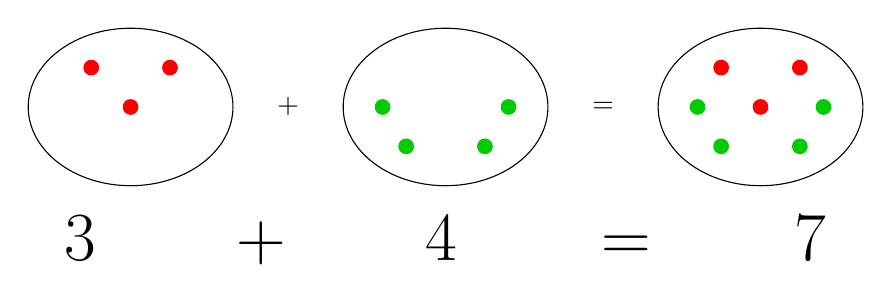
\begin{tikzpicture}
    \draw (0,0) circle (1.3 and 1);
    \node at (2,0) {$+$};
    \draw (4,0) circle (1.3 and 1);
    \node at (6,0) {$=$};
    \draw (8,0) circle (1.3 and 1);

    \fill[red] (0,0) circle (0.1);
    \fill[red] (0.5,0.5) circle (0.1);
    \fill[red] (-0.5,0.5) circle (0.1);

    \fill[green!80!black] (4.8,0) circle (0.1);
    \fill[green!80!black] (3.2,0) circle (0.1);
    \fill[green!80!black] (4.5,-0.5) circle (0.1);
    \fill[green!80!black] (3.5,-0.5) circle (0.1);

    \fill[red] (8,0) circle (0.1);
    \fill[red] (8.5,0.5) circle (0.1);
    \fill[red] (7.5,0.5) circle (0.1);
    \fill[green!80!black] (8.8,0) circle (0.1);
    \fill[green!80!black] (7.2,0) circle (0.1);
    \fill[green!80!black] (8.5,-0.5) circle (0.1);
    \fill[green!80!black] (7.5,-0.5) circle (0.1);

    \node at (4,-1.7) {\Huge $3~~~~~~+~~~~~~4~~~~~~=~~~~~~7$};
\end{tikzpicture}

\end{document}